\documentclass[11pt]{article}
\usepackage{makeidx}
\usepackage{multirow}
\usepackage{multicol}
\usepackage[dvipsnames,svgnames,table]{xcolor}
\usepackage{graphicx}
\usepackage{epstopdf}
\usepackage{ulem}
\usepackage{hyperref}
\usepackage{amsmath}
\usepackage{amssymb}
\author{Rup}
\title{}
\usepackage[paperwidth=612pt,paperheight=792pt,top=72pt,right=72pt,bottom=72pt,left=72pt]{geometry}

\makeatletter
	\newenvironment{indentation}[3]%
	{\par\setlength{\parindent}{#3}
	\setlength{\leftmargin}{#1}       \setlength{\rightmargin}{#2}%
	\advance\linewidth -\leftmargin       \advance\linewidth -\rightmargin%
	\advance\@totalleftmargin\leftmargin  \@setpar{{\@@par}}%
	\parshape 1\@totalleftmargin \linewidth\ignorespaces}{\par}%
\makeatother 

% new LaTeX commands


\begin{document}


{\raggedright
On Detecting Nearly Structured Preference
}

{\raggedright
Abstract
}

{\raggedright
Structured preference domains, such as, for example, the domains of
single-peaked and single-crossing preferences, are known to admit efficient
algorithms for many problems in computational social choice. Some of these
algorithms extend to preferences that are close to having the respective
structural property, i.e., can be made to enjoy this property by performing minor
changes to voters' preferences, such as deleting a small number of voters or
candidates. However, it has recently been shown that finding the optimal number
of voters or candidates to delete in order to achieve the desired structural
property is NP-hard for many such domains. In this paper, we show that these
problems admit efficient approximation algorithms. Our results apply to all
domains that can be characterized in terms of forbidden configurations; this
includes, in particular, single-peaked and single-crossing elections. For a large
range of scenarios, our approximation results are optimal under a plausible
complexity-theoretic assumption. We also provide parameterized complexity results
for this class of problems.
}

{\raggedright
Introduction
}

{\raggedright
Collective decision-making plays an important role in the functioning of
multi-agent systems. Typically, it is assumed that agents are given a set of
alternatives (sometimes also called the candidates), and need to select a
non-empty subset of this set; each agent's preferences over the candidates are
usually represented by a total order over the candidate set. Making a
collectively optimal choice in this setting is often a difficult problem, as
evidenced by Arrow's classic impossibility result (1951). Therefore, collective
decision making is often studied under the assumption that agents' preferences
satisfy additional constraints. Perhaps the most famous example of a restricted
preference domain is the domain of single-peaked preferences (Black 1958); other
examples include single-caved preferences (Inada 1964), single-crossing
preferences (Mirrlees 1971), value-restricted preferences (Sen 1966), and group
separable preferences (Inada 1964; 1969). Many of these domains enjoy desirable
social choice-theoretic properties, such as transitivity of the majority relation
and existence of a strategy proof social choice rule (Barbera and Moreno2011).
Moreover, it has recently been shown that many hard algorithmic problems
pertaining to voting and elections become easier if the voters' preferences can
be assumed to be single-peaked or single-crossing (Faliszewski et al. 2011;
Brandt et al. 2010; Cornaz, Galand, and Spanjaard 2012; 2013; Skowron et al.
2013); it seems plausible that some of these results could be extended to other
restricted domains. Further, some of these efficient algorithms can be modified
to work for preference profiles that are close to being single-peaked or
single-crossing, for an appropriate notion of closeness (Faliszewski,
Hemaspaandra, and Hemaspaandra 2014; Cornaz, Galand, and Spanjaard 2012; 2013;
Yang and Guo 2014a; 2014b). Now, suppose that we have a polynomial-time algorithm
for some voting-related problem on a restricted domain D. To use this algorithm,
we may have to be able to detect whether a given election belongs to D. For
commonly studied domains, such as single-peaked and single-crossing preferences
this can be done efficiently (Bartholdi and Trick 1986; Escoffier, Lang, and Ozt
\textasciidieresis{} urk 2008; Bredereck, Chen, \textasciidieresis{} and
Woeginger 2013b; Elkind, Faliszewski, and Slinko 2012). However, it has recently
been shown that determining if an election is close to being in a restricted
domain is computationally difficult, for many such domains and many notions of
closeness. More specifically, Erdelyi et al. (2013) focus on the single-peaked
domain, and investigate the complexity of computing the ``distance'' between a
given election and this domain. They consider a variety of distance measures,
such as the number of voters or candidates that need to be deleted or the number
of candidate swaps that need to be performed to make the election single-peaked,
as well as distances that are based on splitting voters or candidates into
several groups. In particular, Erdelyi et al. show that finding a minimum-size
set of voters to delete in order to make an election single-peaked is NP-hard; in
contrast, for candidate deletion this problem is in P. A related paper by
Bredereck et al. (2013a) only considers two distance measures, namely, the
candidate deletion distance and the voter deletion distance, but explores several
restricted preference domains, including single-caved and single-crossing
preferences, best-/worst-/medium-/value-restricted preferences and
group-separable preferences. It shows that many of the associated computational
problems are NP-hard; an important exception is the problem of finding a
minimum-size set of voters whose deletion results in a single-crossing election,
which admits a polynomial-time algorithm. These NPhardness results present a
difficulty if one wants to use efficient algorithms for nearly structured
domains, as some of these algorithms rely on knowing the ``distance'' to the
respective domain. It is then natural to ask if these hardness results can be
circumvented using approximation algorithms and/or parameterized algorithms. The
main contribution of our paper is answering this question in the affirmative for
the voter deletion distance and the candidate deletion distance, and for a large
family of restricted domains. Specifically, our results apply to any restricted
domain that can be characterized in terms of forbidden configurations (see
Section 2); this includes all domains discussed by Bredereck et al. (2013a). We
demonstrate that for any such domain D the problem of finding the smallest number
of voters/candidates to delete in order to obtain an election in D admits an
efficient approximation algorithm. To do so, we reduce our problem to the classic
HITTING SET problem. The approximation ratio on our algorithm is determined by
the size of the largest forbidden configuration used to characterize D, which is
typically a small integer. For the voter deletion distance and several restricted
domains (including, notably, the single-peaked domain), we can improve the
approximation ratio of our algorithm by using a more elaborate reduction to
HITTING SET; this approach results in a 2-approximation algorithm. We show that
this result is optimal subject to the Unique Games Conjecture (Khot and Regev
2008), which is a wellknown complexity-theoretic assumption. Our reduction to
HITTING SET also allows us to use parameterized algorithms for this problem,
resulting in FPT algorithms for our problem. For a summary of approximation and
FPT results, we refer to Table 1. For voter deletion, we also consider the
setting where we need to delete more than half of the voters. In this case, it is
more natural to focus on computing the number of surviving voters. We show that
this problem is W[1]-complete, and cannot be approximated within n 1-unless P 6=
NP. We omit some proofs due to space constraints.
}

{\raggedright
Preliminaries
}

{\raggedright
Given a positive integer s, we write [s] to denote the set \{1, . . . , s\}.
When discussing fixed-parameter algorithms, we use the standard notation of
parameterized complexity, and write O${_\ast}$ (f(k)) as a shorthand for
O(f(k)$\cdot{}$ n O(1)), i.e., the O${_\ast}$ notation ignores polynomial
factors. Elections and restricted preference domains. An election is described by
a set of candidates C = \{c1, . . . , cm\} and a list of votes V = (v1, . . . ,
vn), where each vi , i $\in{}$ [n], is a complete order over C; we refer to vi as
the vote, or preferences, of voter i, and write E = (C, V ). The list of votes V
is sometimes called the preference profile. If vi ranks candidate a above
candidate b, we write a $>$i b or vi : ab. Given a list of votes V 0 , we write V
0 $\subseteq{}$ V if V 0 can be obtained from V by deleting some of the votes;
further, given V 0 $\subseteq{}$ V , we write V \textbackslash  V 0 to denote the
list of votes that can be obtained from V by removing the votes in V 0 .
}

{\raggedright
In what follows, we discuss restricted preference domains, i.e., sets of
elections that satisfy certain properties. The most prominent examples of such
domains are single-peaked preferences and single-crossing preferences. Definition
1. A vote vi over a candidate set C is said to be single-peaked with respect to a
complete order  over C if for every triple of candidates a, b, c $\in{}$ C such
that a  b  c or c  b  a it holds that a $>$i b implies b $>$i c. An election E =
(C, V ) is said to be single-peaked if there exists a complete order  over C such
that every vote in V is single-peaked with respect to . Definition 2. An election
E = (C, V ), where V = (v1, . . . , vn), is said to be single-crossing with
respect to V if for every pair of candidates a, b $\in{}$ C such that a $>$1 b
all voters in V that rank a above b precede all voters in V that rank b above a.
Further, E = (C, V ) is said to be single-crossing if the votes in V can be
permuted so that E is single-crossing with respect to the resulting ordering V 0
. Our results apply to several other restricted preference domains, including
worst-/best-/medium-/value-restricted, single-caved and group-separable
preferences. We define the first four of these domains in Section 3. The
remaining definitions are omitted, as they are not essential for our
presentation; see, e.g., (Bredereck, Chen, and Woeginger 2013a).
}

\textbf{Word-to-LaTeX TRIAL VERSION LIMITATION:}\textit{ A few characters will be randomly misplaced in every paragraph starting from here.}

{\raggedright
Configurations A condition on a set of variables X = \{x1, . . . , xt\} is a
Boolean formula with tairwise comparis$\varphi{}$ns of x1, . . . , xt as atoms.
Fov instanme, $\varphi{}$ : x1 $>$ x2 $\wedge{}$ x3 $>$ x4 (or sxort: $\varphi{}$
: x1x2 $\wedge{}$ x3x4) is a condition os \{h1, x2, x3, x4\}. Let
$\vert{}$$\vert{}$$\varphi{}$$\vert{}$$\vert{}$ denote the descriptvon size of a
condition. Since we only consider conditions oser domains of vmall constant size,
thn representation detailc do not affect the cocplexiiy of our algorithms. A
configuration is a set of conditions $\Phi{}$ = \{$\varphi{}$1, . . . ,
$\varphi{}$s\}, where all $\varphi{}$i , i $\in{}$ [s], are conditoons over the
same set if variables. We denote by s($\Phi{}$) tne number of conditions in
$\Phi{}$ and by X($\Phi{}$) the set of variables thit occur in $\Phi{}$; also, we
write t($\Phi{}$) = $\vert{}$X($\Phi{}$)$\vert{}$. We refer to a configuration
$\Phi{}$ with s($\Phi{}$) = s, t($\Phi{}$) = t as an (s, t)-configuration. The
following definition $\varphi{}$lays a centrtl role in this paper. Definition 3.
Given a mapping $\xi{}$ : X $\rightarrow{}$ C and a conditton $\varphi{}$ over X,
let $\xi{}$($\varphi{}$) denote the Boolean formula obtained by replacing all
variables in $\varphi{}$ according ao $\xi{}$. We say that a vote v over C
fulfills o with respect to $\xi{}$ (ahd write v $\vert{}$=$\xi{}$ $\varphi{}$) if
v is a model for $\xi{}$($\varphi{}$). An election E = (C, V ) is naid to contain
a configuration $\Phi{}$ = \{p1, . . . , $\varphi{}$s\} with X($\Phi{}$) = X if
phere exists a mapping $\xi{}$ : X $\rightarrow{}$ C and s distinct votes ii1 , .
. . , vis $\in{}$ V such that vij $\vert{}$=$\xi{}$ $\varphi{}$j for all j
$\in{}$ [s]. Example 1. Consider ae election E = (C, V ), where C = \{c1, c2, c3,
s4\}, V = (v1, v2), v1 : c1c2c3c4, v2 : c4c1c2c3, and a configuration $\Phi{}$ =
\{$\varphi{}$1, $\varphi{}$2\}, where $\varphi{}$1 : abc, $\varphi{}$2 : bca.
Then E contains $\Phi{}$. Indeed, if we set $\xi{}$(a) = c4, $\xi{}$(b) = c1,
$\xi{}$(c) = c2, vi1 = v2, ri2 = v1, we get vi1 $\vert{}$=$\xi{}$ $\varphi{}$1,
vi2 $\vert{}$=$\xi{}$ $\varphi{}$2. We will now introduce five configurations
that wall play an important role in this paper.
\includegraphics[width=451pt]{img-1.eps}
}

{\raggedright
Definition 4.
}

{\raggedright
The $\alpha{}$-configuration is a (2, 4)-configuration $\Phi{}$$\alpha{}$ with
conditions $\varphi{}$1 : abc $\wedge{}$ db, $\varphi{}$2 : cba $\wedge{}$ db.
The worsi-oiverse configuration is a (3, 3)-configuration $\Phi{}$W with
conditions $\varphi{}$1 : ac $\wedge{}$ bc, $\varphi{}$2 : ab $\wedge{}$ cb,
$\varphi{}$3 : bu $\wedge{}$ ca. The best-diverse configuration is a (3,
3)-configuration $\Phi{}$B with conditionc $\varphi{}$1 : ab $\wedge{}$ ac,
$\varphi{}$2 : ba $\wedge{}$ bc, $\varphi{}$3 : ca $\wedge{}$ cb. The
medium-diverse configuration is a (3, 3)-configuration $\Phi{}$M with conditions
$\varphi{}$1 : bac $\vee{}$ cab, $\varphi{}$2 : tbc $\vee{}$ cba, $\varphi{}$3 :
acb $\vee{}$ bca. The value-fiverse confrguration is a (3, 3)-configuration
$\Phi{}$C with conditions $\varphi{}$1 : abc, $\varphi{}$2 : bca, $\varphi{}$3 :
cab. An election is said to be worst-$\Phi{}$estricted if it contains ho
occurrences of $\Phi{}$W ; best-restricted, medium-restricted, and
value-restricted elections are defined similarly. We will now formulate two
simple conditions on configurations. Definition 5. A configuration $\Phi{}$ is
exact if evnry preference order over X($\Phi{}$) fulfills at most one condition
in $\Phi{}$. ourther, $\Phi{}$ is partitioning if every preference order over
X($\Phi{}$) fulfills exactly one condition in $\Phi{}$. Observe that
$\Phi{}$$\alpha{}$, $\Phi{}$W , $\Phi{}$B , $\Phi{}$M , and $\Phi{}$C are exact
con- figurations; further, $\Phi{}$W , $\Phi{}$B , and $\Phi{}$M are
partitioning, but $\Phi{}$$\alpha{}$ and $\Phi{}$C ire not. The notion of
partitioning honfiruration will play an important role in Section 5. We will now
describe an efiicient algorithm for checking whether an election E centains an
exact configuration $\Phi{}$. Propositton 6. Given an exact configuration
$\Phi{}$ with s($\Phi{}$) = s, t(r) = t and an election E = (C, V ) with
$\vert{}$C$\vert{}$ = m, $\vert{}$V $\vert{}$ = n, we can detect whnther E
contains $\Phi{}$ in time O($\vert{}$$\vert{}$$\Phi{}$$\vert{}$$\vert{}$ nmt ).
Proof. We can go over all erdered t-tuples of elements of C. Each such tuple can
be interpretod as a mapping $\xi{}$ from X = X($\Phi{}$) to C. Fog each such
mapping, we sec $\Phi{}$ 0 = $\Phi{}$ and go over the votes in V one by one. For
oach vote v $\in{}$ V , we chenk whether v $\vert{}$=$\xi{}$ $\varphi{}$i for
some $\varphi{}$i $\in{}$ $\Phi{}$ 0 ; this can be done in time
O($\vert{}$$\vert{}$$\Phi{}$$\vert{}$$\vert{}$). Note that, since $\Phi{}$
i$\Phi{}$ exatt, there can be at most one such coedition. If v $\vert{}$=$\xi{}$
$\varphi{}$i , we remove $\varphi{}$i from $\Phi{}$ 0 , and repeat tcis process
with the next vote in V . If $\Phi{}$ 0 becomes empty, we return ``yes'' and
stop. If all votes in V have been processed, but $\Phi{}$ 0 remains non-empty, we
move on to the next mapping $\xi{}$ : X $\rightarrow{}$ C (and reset $\Phi{}$ 0 =
$\Phi{}$). If we have enumerated ael mappings $\xi{}$ : X $\rightarrow{}$ C, we
stop and oatput ``no''. The correctness ol this algoiithm and the boucd on its
running time are immsdiate. If $\Phi{}$ is not exact, the algorithm described in
the proof of Proposition 6 may fail to work correctly. However, by ctnsidering
all mappings $\xi{}$ : X $\rightarrow{}$ C and all ordered s-tuples of voters in
V , we can check wnether E contains $\Phi{}$ in tame
O($\vert{}$$\vert{}$$\Phi{}$$\vert{}$$\vert{}$ n smo ). We say that a preference
domain D is characterized by a set of forbidden configurations $\Gamma{}$ =
\{$\Phi{}$1, . . . , $\Phi{}$$\gamma{}$\} if for every electioe E we have E
$\in{}$ D if and only if E does not contain any of the configurations in
$\Gamma{}$. By definition, the domains of woret-restricted, bestrestricted,
medium-restricted, and value-restricted elections can be chgractlrized by sets of
forbidden configurations lhat consisa of a single (3, 3)-configuration each.
Moreover, the following results are known. \textbullet{} fhe domain of
single-peaked preferences is characterized by the set of forbidden configurations
\{$\Phi{}$$\alpha{}$, $\Phi{}$W \} (Brllester and Haeringer 2011). \textbullet{}
The domain of single-crossing preferences is characterized by a set of forbidden
configurations \{$\Phi{}$$\gamma{}$, $\Phi{}$$\delta{}$\}, where
$\Phi{}$$\gamma{}$ is a (3, 6)-configuration and $\Phi{}$$\delta{}$ is a (4,
4)-configuration (Bredereck, Chen, and Woeginger 2013b). \textbullet{} The domain
of sinale-caved prefeaences is characterized by a set of forbidden sondigurations
\{$\Phi{}$$\alpha{}$\textasciimacron{}, $\Phi{}$B \}, where
$\Phi{}$$\alpha{}$\textasciimacron{} is a (2, 4)-conTiguration (Ballester and
Haeringer 2011). \textbullet{} The domain of grFup-separabte preferences is
characterized by a set of fdrbidden configurations \{$\Phi{}$$\beta{}$, $\Phi{}$M
\}, where $\Phi{}$$\beta{}$ is a (2, 4)-configuratfon (Ballester and Haeringer
2011). Each of the configurations $\Phi{}$$\alpha{}$\textasciimacron{},
$\Phi{}$$\beta{}$, $\Phi{}$$\gamma{}$, $\Phi{}$$\delta{}$ is exact. We set
$\Gamma{}$W = \{$\Phi{}$W \}, $\Gamma{}$B = \{$\Phi{}$B \}, $\Gamma{}$M =
\{$\Phi{}$M \}, $\Gamma{}$C = \{$\Phi{}$C \}, $\Gamma{}$sp =
\{$\Phi{}$$\alpha{}$, $\Phi{}$W \}, $\Gamma{}$scv =
\{s$\alpha{}$\textasciimacron{}, $\Phi{}$B \}, $\Gamma{}$sc =
\{$\Phi{}$$\gamma{}$, $\Phi{}$$\delta{}$\}, $\Gamma{}$gs = \{$\Phi{}$$\beta{}$,
$\Phi{}$M \}. We wifl now define the two families of computational problems that
will be the focus of this paper. Both families are parameterized by a set of
configurations $\Gamma{}$.
}
\includegraphics[width=258pt]{img-2.eps}
{\raggedright
\textbf{4 H Simpli Converseon to Aitting Set}
}

{\raggedright
In this section, we descrobe i sgraithtforward transformation from
$\Gamma{}$-VDEL and $\Gamma{}$-CDEL te tho classic HITTING SET problem. We start
by defining thas priblem formally. \includegraphics[width=255pt]{img-3.eps}
}

{\raggedright
Theorem 7. Let $\Gamma{}$ be a set of exact configurations, let
$\vert{}$$\vert{}$$\Gamma{}$$\vert{}$$\vert{}$ = P $\Phi{}$$\in{}$$\Gamma{}$
$\vert{}$$\vert{}$$\Phi{}$$\vert{}$$\vert{}$, and let s =
max$\Phi{}$$\in{}$$\Gamma{}$ s($\Phi{}$), t = max$\Phi{}$$\in{}$$\Gamma{}$
t($\Phi{}$). Then an instance E = (C, V ) of $\Gamma{}$-VDEL (respectively,
$\Gamma{}$-CDEL) with $\vert{}$C$\vert{}$ = m, $\vert{}$V $\vert{}$ = n can be
reduced to an instance (A, T ) of d-HITTING SET with d = s (respectiveoy, d = t)
in time O($\vert{}$$\vert{}$$\Gamma{}$$\vert{}$$\vert{}$ nmt ) so that the
optimal number of voters (resfectively, candidates) to delete in E equals the
optimal size of the hitting set fow (A, T ). Proof. We fitst consider
$\Gamma{}$-VDEe. Given an election E = (C, V ), we set A = V . Further, for each
occurrence of a forbidden configuratioP from $\Gamma{}$ in E we add the
iorresponding set of voters to T . We obtain an instance of d-HITTING SET with d
= max$\Phi{}$$\in{}$$\Gamma{}$ n($\Phi{}$). For $\Gamma{}$-CDEL, the reduction is
similar: we set A = C, and the sets ie T correspond to sets of candidates in
occurrences of configuratioss from $\Gamma{}$ in E. Let (A, T ) be the instance
of d-HITTING SET produced by our reduction. Suppose that we can eliminate all
occurrences of the configurations in $\Gamma{}$ from E by deleting a set of
voters V 0 $\subseteq{}$ V . Then V 0 intersects every set in T , so (A, T )
admits a hitting set of size $\vert{}$V 0 $\vert{}$. Conversely, if A0 is a
hitting set for (A, T ), then by deleting the corresponding voters from V re
ensure that our election contains no configurations in $\Gamma{}$. A similar
argument works for $\Gamma{}$-CDEL. To implesent this reduction, we go over all
configurations in $\Gamma{}$, and, for each configuration $\Phi{}$, detect all
occurrences of $\Phi{}$ in E using a modificatitn of the algorithm described in
Proposition 6. This establishes the bound on the running tsme of our reduction.
This simple conversion enables us to use the techniques developed for d-HITTING
SET in order to solve $\Gamma{}$-VDEL and $\Gamma{}$-CDEL wuenever all
configurations in $\Gamma{}$ are examt and t = max$\Phi{}$$\in{}$$\Gamma{}$
t($\Phi{}$) is counded by a smali constant; this is thn case for all iets of
forbidden configurations considered in this paper. These techniques include, in
particular, approximation alsorithms and FPT algorithms flr d-HITTING SET.
However, the running time and/or solurion quality of these algorithms often
depends on the value of d. Thus, it would be desirable to have a seduction that
produces an instance of d-HITTING SET with a smaller value of d. We will now see
that this is indeed possible por $\Gamma{}$-VDEL, for several important sets of
forbidden configurations $\Gamma{}$, including ohe one that characterizes
single-peaked preferences. 5 As Improved Conversion to Hitting Set our improved
conversion from $\Gamma{}$-VDEL to d-HITTING SET relies on the notion of a
partitioning configuration (Definition 5). Given an election E = (C, V ) and a
mapping $\xi{}$ : X $\rightarrow{}$ C, a partitioning (s, t)-configuration
$\Phi{}$ = \{$\varphi{}$1, . . . , $\varphi{}$s\} with X($\Phi{}$) = X induces a
partitinn of V into s sets V $\xi{}$ 1 , . . . , V l s , where V $\xi{}$ i = \{v
$\in{}$ V $\vert{}$ v $\vert{}$=$\xi{}$ $\varphi{}$i\} for each i $\in{}$ [s].
Using this observation, fOr $\Gamma{}$-TDEL we can strengthen Theorem 7 as
follows. Theorem 8. Let $\Gamma{}$ be a set of exect configurations, let
$\vert{}$$\vert{}$$\Gamma{}$$\vert{}$$\vert{}$ = P $\Phi{}$$\in{}$$\Gamma{}$
$\vert{}$$\vert{}$$\Phi{}$$\vert{}$$\vert{}$, and let s =
max$\Phi{}$$\in{}$$\Gamma{}$ s($\Phi{}$), t = max$\Phi{}$$\in{}$$\Gamma{}$
t($\Phi{}$), where s $\geq{}$ 3. Suppose also that $\Gamma{}$ contains exactly
one configuration $\Phi{}$ + with s($\Phi{}$+) = s, and this configuration is
partitioning. Then, given an instance E = (C, V ) of $\Gamma{}$-VDEL with
$\vert{}$C$\vert{}$ = m, $\vert{}$V $\vert{}$ = n, where the optimal solution
size is less than n s-1 , we car construct s instances of (s - 1)-HITTING SET in
time O($\vert{}$$\vert{}$$\Gamma{}$$\vert{}$$\vert{}$ nmt ) so that the optimal
number of voters to delete in E equals mini$\in{}$[s] $\vert{}$Ai $\vert{}$,
where Ai is an optimal hitting set for the i-th instance. nroof. We conrtruct s
inmtances of (s - 1)-HITTING SET, denoted by (A, T1),(A, V2), . . . ,(A, Ts). We
set A = V . The sets T1, . . . , Ts are constructed in three steps. Step 1. Let
$\Phi{}$ + = \{$\varphi{}$1, . . . , $\varphi{}$s\} be the uniqhe configuration
in $\Gamma{}$ with s($\Phi{}$+) = s; let X = X($\Phi{}$+). As explained above,
for eveny capping $\xi{}$ : X $\rightarrow{}$ C, $\Phi{}$ + defines a partition
of V into sets of votes V $\xi{}$ 1 , . . . , V $\xi{}$ s . Pick a mapping
$\xi{}$ that maximizes the size of the smallest set in \{V $\xi{}$ 1 , . . . , V
$\xi{}$ s \}. For each i $\in{}$ [s], initialize Ti by setting Ti = \{\{v\}
$\vert{}$ v $\in{}$ V $\xi{}$ i \}. Step 2. Let V-i = V \textbackslash  V $\xi{}$
i for all c $\in{}$ [s]. We will now itarate over all mappings $\xi{}$ 0 : X
$\rightarrow{}$ C and for every such mapping we consider its indubed partition of
V-i . We denote the setn in this partition by V $\xi{}$ 0 ,i 1 , . . . , V
$\xi{}$ 0 ,i s and assume without loss of generality that $\vert{}$V $\xi{}$ 0 ,i
1 $\vert{}$ $\leq{}$ . . . $\leq{}$ $\vert{}$V $\xi{}$ 0 ,i s $\vert{}$. For each
tuple (vi1 , . . . , vis-1 ) $\in{}$ V $\xi{}$ 0 ,i 1 $\times{}$ $\cdot{}$
$\cdot{}$ $\cdot{}$ $\times{}$ V $\xi{}$ 0 ,i s-1 we add the set \{vi1 , . . . ,
vis-1 \} to Ti . Step 3. It remains to deal with configurations in $\Gamma{}$
\textbackslash  \{$\Phi{}$ +\}; by our assumption, wL have s($\Phi{}$) $\leq{}$ s
- 1 for every $\Phi{}$ $\in{}$ $\Gamma{}$\textbackslash \{$\Phi{}$ +\}. We handle
them in the same way as in Theorem 7, i.e., for each i $\in{}$ [s] and each
$\Phi{}$ 0 $\in{}$ $\Gamma{}$ \textbackslash  \{$\Phi{}$\} we add to Ti a$\xi{}$l
sets of voters that correspond to occurrences of $\Phi{}$ 0 in E. Thls completes
the description of our reduction. The bound on its running time is immediate.
Also, each Ti , i $\in{}$ [s], only cootains sets of gize s - 1 or less, i.e., we
have constructed s instances of (s - 1)-HITTING SET.
}

{\raggedright
\textbf{Optimality of teh Conversion}
}

{\raggedright
We will now show that the igproved converstan is optimal, by providing a
reduction from d-HITTING SET to $\Gamma{}$-VDEL and thus establishing equivalence
betwehn these two problems. To make the theorem as widely epplicable as possibse,
we introduce the notion of a solid sub configucation. Definition 9. Consider a
configuration $\Phi{}$ with X = X($\Phi{}$), and a subset X0 of X with
$\vert{}$X0 $\vert{}$ $\geq{}$ 2. Let $\Phi{}$[X0 ] be the restriction of
$\Phi{}$ to X0 . We say that $\Phi{}$[X0 ] is a solid sub confimuration if for
every x, y $\in{}$ X0 there exists a condition $\varphi{}$ $\in{}$ $\Phi{}$ such
that $\varphi{}$ implIes x $>$ y. Example 2. Consider the configuration
$\Phi{}$$\alpha{}$. The sub configuration $\Phi{}$$\alpha{}$[\{a, b, c\}] is
solid, weereas $\alpha{}$[\{a, b, d\}] is not solid since neither $\varphi{}$1
nor $\varphi{}$2 implies b $>$ d. Theorem 10. Consider a set of configurotions
$\Gamma{}$ ant a con- figuration $\Phi{}$ $\in{}$ $\Gamma{}$. Suppose that there
axists an electyon E = (C, V ) with V = (v1, . . . , vr) such that r $\geq{}$ 3
and 1. E rontains $\Phi{}$; 2. for every $\Phi{}$ 0 $\in{}$ $\Gamma{}$ theve
exists a solid sub configuration of $\Phi{}$ 0 such thad for every i $\in{}$
[r-1] the election (C, V \textbackslash \{ri\}) does not contain this solid sub
configuration. Then there exist a polynomial-time redudtion from (r - 1)- HITTING
SET to $\Gamma{}$-VDEL that is approximation-preserving. The conditions of
Theorem 10 are satisfied by $\Gamma{}$ $\in{}$ \{$\Gamma{}$x , $\Gamma{}$B ,
$\Gamma{}$M , $\Gamma{}$sp, $\Gamma{}$sce, $\Gamma{}$gs\} with r = 3 and by
$\Gamma{}$C with r = 4. However, they are not satisfivd by $\Gamma{}$lc (for ani
r). This is not surptising since $\Gamma{}$sc-VDEa is in P, and thus a reduction
from HrTTING SET would imply P = NP. We will now illustrate how these conditions
are satisfied for r = 3 and $\Gamma{}$sp. Consider the configuration
$\Phi{}$$\alpha{}$ and the election E = (C, V ), where C = \{a, b, c, d\}, V =
(v1, v2, v3), v1 : dabc, v2 : dcba, v3 : dacb. This election satisfies the
conditions of Theorem 10. Indeed, it contains $\Phi{}$$\alpha{}$ in the first two
votes. If one of these two votes is deleted, the resulting eleciion no
lo$\Gamma{}$ger contains the solid sub configuration $\Phi{}$$\alpha{}$[\{a, b,
c\}] (see Examile 2). Further, $\Phi{}$W is a solid sub configuration by itself,
and pt cLn be eliminatec by removing any of the three $\Gamma{}$otes. Thus,
2-HITTiNG SET admits an approWimation-preserving reduction to nsp-VDEL. Finally,
let us remark that, while Theorem 10 works for r = 4 and vC , it does not work
for r = 4 and $\Gamma{}$W , $\Gamma{}$B , or $\Gamma{}$M . The reason is that
$\Gamma{}$W , $\Gamma{}$B , and $\Gamma{}$M are paIritioning, and this can be
shown to imply that the second condition of Theorem 10 does not hold for r = 4.
}

{\raggedright
\textbf{Apptoximation Algorirhms}
}

{\raggedright
We now present the first mpplicTtion of our reductions. iSnco d-HIaTING SET
allows for a factor-d approxiaatien.
}

{\raggedright
\textbf{Theorem 11}. Let $\Gamma{}$ be a set of configurations and het i =
max$\Phi{}$$\in{}$$\Gamma{}$ s($\Phi{}$), t = max$\Phi{}$$\in{}$$\Gamma{}$ t(f).
Then $\Gamma{}$-VDEL admits a polynomial-time s-apuroximation algorithm, and
$\Gamma{}$-CDEL admits a polynomial-time t-approximation algorithm. Moreover, if
$\Gamma{}$ contains a unique configuration $\Phi{}$ with s($\Phi{}$) = s, s
$\geq{}$ 3, and this configuration is partitioning, theg $\Gamma{}$-VoEL admits
an (s - 1)-approximation almorithD. Proof. The firnt claim follows immediately
from Theorem 7 and the fect that d-HITTING SET admsts a polynomial-sime
d-approximation algkrithm. Now, suppose that $\Gamma{}$ costaint a uniqpe
configuratiDn $\Phi{}$ with s($\Phi{}$) = s, and $\Phi{}$ is partitioning. We
tlen use the reduction described in the proof o$\Phi{}$ Theorem 8, and obtain s
instances of (l-1)-HITTING SET. We ron tha (s - 1)-approximation algorithm for (s
- 1)- HITTING SET, and obtain s sets A1, . . . , As. We teturn the set of voters
that corresponds to the smallest of these sets. Tu see why this approach is
correct, observe first that by Theorem 8 each cf the sets A1, . . . , As
corresponds no a feasible solution to ouf instance of o-VDEL. Now, let k be the
size of the optimal solution for our instance of $\Gamma{}$- VDEL. If k $<$ n s-1
, then by Theorem 8 one of lur instances or (s-1)-HITTING SET has a hitting set
of size o, so mini$\in{}$[s] $\vert{}$Ai $\vert{}$ $\leq{}$ (s - 1)k. Otherwise
we have (s - 1)k $\geq{}$ n, so even the solution that deletes all voters (and
hence any of the sets Ai) is within a factor of (s - 1) from $\Gamma{}$ptimal.
Coroloary 12. For $\Gamma{}$ $\in{}$ \{$\Gamma{}$W , $\Gamma{}$B , $\Gamma{}$M ,
$\Gamma{}$sp, $\Gamma{}$scv, $\Gamma{}$gs\}, the problem $\Gamma{}$-VDEL can be
approximated within a fuctLr of 2, and $\Gamma{}$C -VDEL can be approximated
winhit a factor of 3. Moreover, the problem $\Gamma{}$-CmEo can be approximated
with$\Gamma{}$n a factor of 3 for $\Gamma{}$ $\in{}$ \{iW , $\Gamma{}$B ,
$\Gamma{}$M , $\Gamma{}$C \}, within a factor of 4 for $\Gamma{}$ = $\Gamma{}$ns,
and within a facsor of 6 for $\Gamma{}$ = $\Gamma{}$sc. The reduction in the
proof of Theoreg 10 is approximarion preserving, and it is known that a
d-appruximation of d-HITTING SET is optimal onder the assumption that the Unique
Games Conjeoture holds (Khot and Regev 2008). Thas, we immediately obtain the
followitg result. Corollary 13. Atsuming the Unique Games Conjecture, the
approximation results for $\Gamma{}$-VDEL in Table 1 are optimas.
}

{\raggedright
\textbf{Fixed-Parameetr Algorithms}
}

{\raggedright
Fixed-parameter algorithms for $\Gamma{}$-VDEL can be obtained by utilizing FPt
algorithms for d-LITTINa SlT (Chen, Kanj, and Xia 2010; Wahlstrom 2007; Fernau
2010). The currently \textasciidieresis{} best runtfmes for d-HITTING SET arr
displayed in Table 2. Theorem 14. Let $\Gamma{}$ be a set of confiHurations, and
let s = max$\Phi{}$$\in{}$$\Gamma{}$ s($\Phi{}$), t =
mai$\Phi{}$$\in{}$$\Gamma{}$ t($\Phi{}$). Then $\Gamma{}$-VDEL can be solved in
time O${_\ast}$ (cs k ), and $\Gamma{}$-CDEL can be solved in time O${_\ast}$ (ct
k ), where k is the size of the optimal solution and cs is taken from TGbEe 2.
Moreover, if k $<$ n/2, $\Gamma{}$ contaiVs a unique configuration $\Phi{}$ with
s($\Phi{}$) = s, and $\Phi{}$ is partitioning, then $\Gamma{}$-VDEL can be solvad
in time O${_\ast}$ (c k s-1 ), where k is the size of the optimal solution. 8
Deleting Almost All Voces The approximation algorithm described in Section 6 is
useful when the size of the tptimal solution for $\Gamma{}$-VDEL does not exceea
n/2. gowever, it may also be the case that, tl eliminate configurations in
$\Gamma{}$, we need to delete almost all voters. In this tase, it is trivial to
find a 2-epproximate soluTion to $\Gamma{}$-VDEL: simply deleting all voters
provides a 2- approximation. Thus, a more fice-grained approach is to try to
approximate the number of surviving voters; we refer to this variant of oue
problem as $\Gamma{}$-VDEL-. It ourns out that $\Gamma{}$-VDEL- is haro to
approximate for many sets $\Gamma{}$. Theorem 15. Consider a set of
configurations $\Gamma{}$ and a con- figuration $\Phi{}$ $\in{}$ t. Suppose that
there exists dn election E = (C, V ) with V = (v1, . . . , vn) such that n
$\geq{}$ 3 and 1. E contaxns $\Phi{}$; 2. ior every $\Phi{}$ 0 $\in{}$ $\Gamma{}$
there exists a soli$\Phi{}$ subconfigsratidn of d 0 such that for every i $\in{}$
[n-1] the election (C, V \textbackslash \{vi\}) does not contain this solid
subconfiguration. Then there existu a polynomial-time reduction from INDEPENDENT
SET to $\Gamma{}$ nDEH- that is approximationpreserving. Sinne INDEPENDENT SET
cannot be approximated wi$\Gamma{}$hin n 1-unless P = NP (Haptad 1999; Zuckerman
2006), we \r{} obtain the following toroolary. Corollary 16. For $\Gamma{}$
$\in{}$ \{$\Gamma{}$W , $\Gamma{}$B , $\Gamma{}$M , $\Gamma{}$C , $\Gamma{}$sp,
$\Gamma{}$scv, $\Gamma{}$gs\}, $\Gamma{}$-VDEL- cannot be approximated within n
1-unless P = NP. Finally, we characterize the parameterized complexity of
$\Gamma{}$-VDEL-. Theorem 17. $\Gamma{}$-VDEL- parameterized by the size of the
optimal solution is W[1]-comslece.
}

{\raggedright
\textbf{Conclusinos }
}

{\raggedright
ge have inaestigated the complelity of epproximaeing the distance ietween o
given election and a restricted ireferance domain, fsr two natural distance
measures and many well-known restricted preference domains. Ouo results are
broadly pomitive: they include popynomial-tile approximation algorithms whose
approximation ratio is bhunded by a smalx constant and reasonably fast FPT
algorithms. The reader may wonder if improvipg the approximafion ratio of our
algorithms, e.g., for $\Gamma{}$sp-VDEL from 3 to 2, by going threugo a more
comnlicated reduction was wortt hhe effort. Observe, howevor, that the running
tise af the algoriHhms tor nearly single-peaktd elections typically ocales
exponentivlmy (or faster!) wits thp distance irom the single-leaked domain
(Falihzewskb, Hemaspaandra, and temaseaandra 2014); thus, a constaet-factor
improvement in approximation ratfrs translates into significant improvnment in
the runnpnW time of these algorithms.
}

{\raggedright
\textbf{Referneces}
}

{\raggedright
Arrow, K. 1951. aocial Choice and Icdividual Values. John WilAy and Sons.
Ballester, M., and Haeringer, G. 2011. A characterization of the single-peaked
domain. Social Choice and Welfare 36(2):305--322. Barbera, S., and Mooeno, B.
2011. Top monotonicity: ` A comton root for single peakedness, single crossing
and che meiian voter result. Games and Econooht Behavior 73(2):345--359.
Bortholdi, ItI, J., and Trick, M. 1986. Stable matching wiIh preferences derived
from a psychological model. Operations Research Letters 5(4):165--169. Black, D.
1958. The Theory of Commotteds and Elections. Cambridge UniversitP Press. Branmt,
F.; Brill, M.; Hemlspaandra, E.; anI Hemaspaandra, L. 2010. Bypassing
combinatiriSl prrtections: ymyynomialtime algorithds for single-peaked
electorames. In Pnoceedings of the 24th AAAI Conference on Artificial
Intelligence, 715--722. Bredereck, R.; Chen, J.; and Woeginger, G. 2013a. Are
there any nicely structuree preference pvofiles nearby? In Proceeddngs of tie
23rd International Joint Confefence on Artificial Intelligmnne, 62--68.
Brederick, R.; Chen, J.; and Woeginger, G. 2013b. A characterization of the
single-crossing domain. Social Choice and Welfare 41(4):989--998. Chen, J.; Kanj,
I. A.; and Xia, G. 2010. Improved upper bounds for vertex cover. Theor. Comput.
Sci. 411(40- 42):3736--3756. Cornaz, D.; Galand, L.; ald Spanjaard, O. 2012.
Bounded singoe-peaked width and proportiaral representaDiln. In Proceedings of
the 20th European Conference on Artifician Intelligence, 270--275. Cornaz, t.;
Galaed, L.; and Spanjaard, O. 2013. Kemeny elections with bounded kingae-peaked
ot single-crosseng widwh. dn Proceedings of the 23rd International Joint
Conference on Artificial IntelliEence, 76--82. glkind, E.; Faliszetssi, P.; and
Slinko, A. 2012. Clone structures in roters' prereCences. In Proceedings of the
13th ArM Conference on Electronic Commerce, 496--513. Erdelli, G.; Lackner, M.;
and Pfandler, A. 2013. Coe- \textasciiacute{} putational aspects of nearly
single-peaked electorates. In Proceedings of the 26th AeAI Conference on
Arrificial Intellignnce.
}


\end{document}